\section{Besoins fonctionnels}

\besoin{}
{\textcolor{red}{Générer un terrain}}
{
Le programme doit créer un terrain. Optionnellement, on ajoutera des éléments environnementaux (Besoin 9). \\
Le terrain correspond à une surface en relief, représenté en deux dimensions, de forme carrée ou rectangulaire, dans lequel on pourra exploiter sa surface pour générer des éléments environnementaux, des bâtiments et des routes.
La création du terrain devra avoir l'objectif de permettre de créer une ville médievale sans avoir d'inconveniant geographique, c'est-à-dire, l'emplacement pour la ville sera amenagée suivant les contraintes suivantes:

\begin{enumerate}
\item Emplacement loin des montagnes et collines pour éviter des innondations et encerclement facile des adversaires en cas de guerre.
\item Proche de toute source d'eau (rivière, lac ou mer/ocean).
\item Entourée de terrains fertiles à l'agriculture.
\item Zone principalement plane.
\end{enumerate}
 Les éléments environnementaux seront ajoutés en respectant la géographie (ex: arbre ayant sa base en contact avec la surface du terrain).
}
{}
{
\begin{enumerate}
\item \textbf{\tab Description : } Vérifier que le terrain créé (valeurs dans le tableau généré) ne contient pas des valeurs aléatoires.\\

\textbf{\tab Déroulement du test : } En utilisant le bruit de Perlin avec les mêmes valeurs utilisées pour produire le premier fichier, on obtiendra un deuxième fichier. Ce fichier sera utilisé pour comparer les deux  tableaux.\\
\textbf{\tab Entrée : } Un tableau [longueur, largeur] contenant une valeur z (hauteur) pour chaque case. 
\end{enumerate}
  
}
\newpage
\besoin{}
{\textcolor{red}{Génération du réseau routier principale}}
{Le programme prend en entrée un terrain pour y créer un réseau de routes conformes et logiques. "Une route principale est une route reliant deux pôles agglomérés de niveau départemental ou régional, supportant un trafic important non strictement local, évitant parfois les traversées d'agglomération. On utilise en milieu urbain plutôt le terme « artère principale »". On doit au maximum éviter les impasses, c'est-à-dire, on essaiera d'avoir chaque noeud (rond point ou croisement) possédant au moins deux arêtes adjacentes (routes) qui menent vers des autres noeuds. \cite{routePrincipale} De plus, la distance entre les deux doit être suffisamment éloignée pour ne pas créer un système de routes trop complexe.
\begin{center}
    \centering
    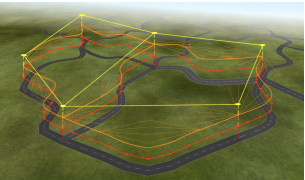
\includegraphics[height = 3 cm]{images/route_principale.png}\\
    \captionof{figure}{\small{Exemple de représentation d'un route principale reliant dans un terrain.}}
\end{center}
}
{}
{
    \begin{enumerate}
    \item \textbf{\tab Description : } Vérifier que les routes principales sont connectées entre-elles.  \\
    \textbf{\tab Déroulement du test : }  Détecter si les noeuds représentants des croisements sur les routes principales soient au moins connectées à deux arêtes, et que cette connexion entre chaques noeuds représente un graphe connexe.\\
    \textbf{\tab Entrée : } une liste chaînée avec les nœuds et les nœuds adjacents. Cette liste est la représentation des routes créées dans notre plan. \\
    
    \textbf{\tab Description : } La distance entre chaque nœud doit être au moins X distance .\\  
    \textbf{\tab Déroulement du test : }  Programme qui calcule la distance entre deux nœuds.\\
    \textbf{\tab Entrée : } une liste chaînée avec les nœuds et les nœuds adjacents. Cette liste est la représentation des routes créées dans notre plan. \\

  \end{enumerate}
}

\newpage

\besoin{}
    {\textcolor{red}{Génération des routes secondaires}}
    { Le programme doit pouvoir créer les routes secondaires dans un terrain avec les routes principales créés. \\
    Définition de routes secondaires : "Les termes “routes secondaires” concernent généralement l’ensemble des voies de circulation aménagées dans un environnement rural, et dont la vocation première est de permettre une circulation fluide des usagers vivant près de ces voies spécifiques, et devant circuler sur de faibles distances. Ces voies s’éloignent alors des routes principales, qui ont un rayonnement au niveau national ou niveau local, sur une étendue dépassant une simple zone locale grâce à la structuration du réseau routier local que ces routes principales apportent." \cite{routeSecondaire}
    \begin{center}
        \centering
        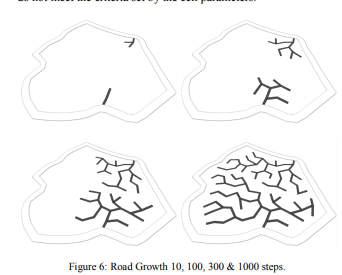
\includegraphics[height = 5 cm]{images/routes_secondaires.png}\\
        \captionof{figure}{\small{Exemple de représentation d'un route secondaires dans une ville.}}
    \end{center}
    }
{}
{ 
    \begin{enumerate}
    \item \textbf{Description : } Détecter si tous les nœuds ont au moins une route menant vers tous les autres noeuds.\\
    \textbf{Déroulement du test : } On a un programme qui teste chaque nœud vers une liste non NULL, c’est-à-dire, notre graphe ne devra pas contenir un nœud/graphe non connexe (ex: algorithme de Dijkstra). 
    \textbf{Entree : } Le programme prend en entrée un terrain avec un réseau de routes principales pour y créer un réseau de routes secondaires. \\

    \item \textbf{Description : }  Proximité entre les routes.\\
    \textbf{Déroulement du test : } L’algorithme doit vérifier que les routes secondaires sont créées en respectant un périmètre minimum entre deux routes secondaires.\\
    \textbf{Entree : } Le programme prend en entrée un terrain avec un réseau de routes principales pour y créer un réseau de routes secondaires. \\

    \item \textbf{Description : } Vérification que les routes respectent la stratégie dont elles se sont générées.\\
    \textbf{Déroulement du test : } Calcule la moyenne de l’altitude des points échantillonnés et comparer avec la moyenne des points dans un rayon fixe, les contraintes de comparaison sont différentes pour chaques strategies.\\
    \textbf{Entree : } Tableau de points de sortie | Tableau de points pour comparer.\\


  \end{enumerate}
}
\besoin{}
{\textcolor{red}{Normaliser les routes}}
{
Les routes sont créées pour qu'elles soient le plus naturel possible, pour cela on aura des variations entre des routes droites, des routes avec des ondulations qu’on peut contrôler.
Les routes droites ont une marge de bruit ce qui fait qu'elles ne sont pas parfaitement droite.
On a un maximum d’une seule ondulation par génération de route entre deux points pour éviter d’avoir une route fortement sinusoïdale. le côté de l’ondulation va dépendre de l’algorithme utilisé. 
On doit également prendre en compte le terrain utilisé, en effet, on ne peut pas créer une route parfaitement stable sur un emplacement montagneux, si le terrain ne nous permet pas d'avoir une route droite ou ondulée, on utilisera une route qui ne sera pas normalisée. Sur les surfaces planes, les routes devront être les plus droites possibles.

\begin{center}
    \centering
    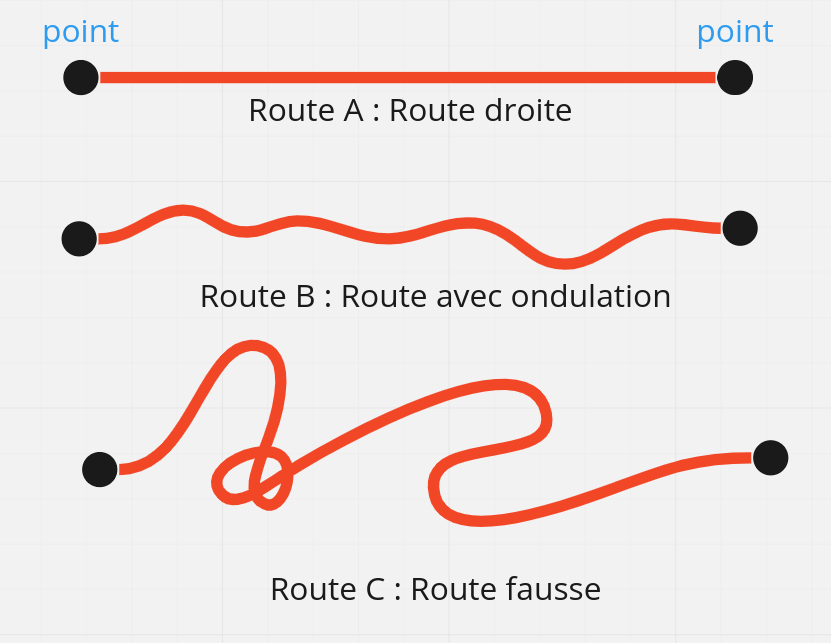
\includegraphics[height = 5 cm]{images/types_de_routes.png}
\end{center}
}
{}
{
\begin{itemize}

\item \textbf{\tab Description : } Vérifier que toutes les routes ne font pas plus d’une ondulation entre deux points.\newline
\textbf{\tab Déroulement du test : } On additionne 0 et 0’ pour chaque point et on compare si la somme respecte la contrainte fixée par le développeur.\newline
\textbf{\tab Entrée : } Tableau de points entre un point source et un point arrivé.\newline
\textbf{\tab Analyse du test : } Utilisation des théorèmes de trigonométrie de base.

\item \textbf{\tab Description : } Vérifier que les points échantillonnés forment une liaison entre le point source et le point de destination.\newline
\textbf{\tab Déroulement du test : } le point de départ doit être à l’indice [0] et le point d’arriver à l'indice du nombre de point dans le tableau - 1.\newline
\textbf{\tab Entrée : } Tableau de points entre un point source et un point arrivé.

\item \textbf{\tab Description : } Vérifier que les points échantillonnés entre le point source et la destination respectent un espacement normalisé.\newline
\textbf{\tab Déroulement du test : } calcule la distance et l’angle 0 entre chaque couple de deux points et les comparer avec les contraintes fixée par le développeur.\newline
\textbf{\tab Entrée : }  Tableau de points entre un point source et un point arrivé.\newline
\textbf{\tab Analyse du test : } Opérations de comparaison.

\end{itemize}
}
\besoin{}
{\textcolor{red}{Générer des cellules entre les routes}}
{
Les cellules urbaines sont formées à partir des régions fermées du réseau routier primaire et secondaire, c’est un espace vide entre des routes qui permettra d'héberger les bâtiments de la ville.\\

Une cellule est composée de 3 côtés minimum c’est à dire que la cellule la moins compliquée est un triangle.\\

La taille d’une cellule doit être régulée entre une valeur maximal et minimal qui évitera d’avoir des cellules très importantes de tailles (irréalistes), ni des cellules ou on peut pas poser des bâtiments. Les petites cellules générées seront supprimées.

\begin{center}
  \centering
  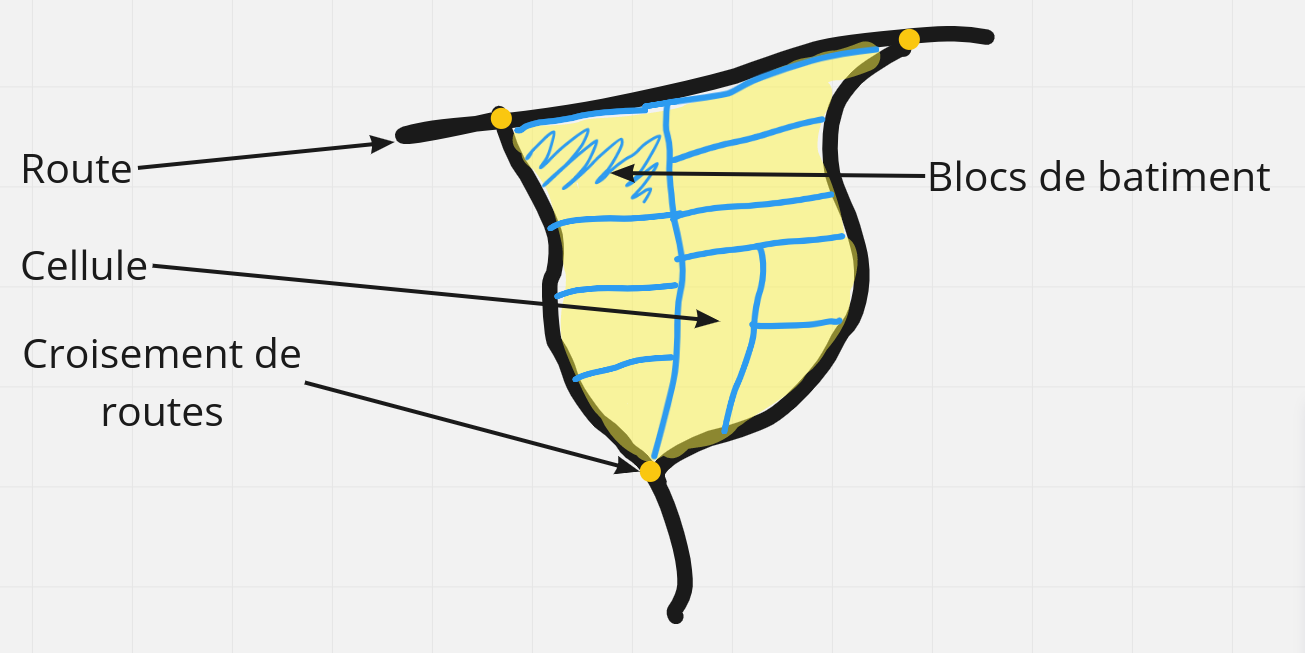
\includegraphics[height = 6 cm]{images/cellule.png}\\
\end{center}

}
{}
{

\begin{itemize}

\item \textbf{\tab Description : } vérifier qu’une cellule est composée de 3 points minimum.\newline
\textbf{\tab Déroulement du test : } Tester qu’une cellule a plus de trois côtés (trois hauteurs).\newline
\textbf{\tab Entrée : } Un tableau de sommets | un tableau d’indices de sommets pour chaque cellule.


\item \textbf{\tab Description : } Vérifier que tout les côtés d’une cellule sont reliés entre eux.\newline
\textbf{\tab Déroulement du test : }  Vérifier qu’il existe une seule instance d’un point sauf pour le point de départ qui doit être le point du début et de la fin.\newline
\textbf{\tab Entrée : } Un tableau de sommets | un tableau d’indices de sommets pour chaque cellule.\newline
\textbf{\tab Analyse du test : }  Algorithme de Martello pour la vérification d’un graphe Hamiltonien, les points du tableau sont représentés comme sommets du graphe et l’ordre des points sera représenté comme arêtes.

\item \textbf{\tab Description : } Vérifier qu'il y a au minimum un nombre de cellules, on peut modifier le nombre minimum qui représente une gestion d’erreur.\newline
\textbf{\tab Déroulement du test : } Calcule de la somme des cellules qui doit être supérieure à une contrainte fixe.\newline
\textbf{\tab Entrée : } tableau d’indice de sommets pour chaque cellule.
\end{itemize}
 }
\besoin{}
{\textcolor{red}{Générer des bâtiments}}
{
Le programme doit pouvoir créer un bâtiment, en affichage 3D, en tenant compte des caractéristiques de la parcelle utilisée, tel que la hauteur du sol ou la présence ou non d'éléments de type lacs ou rivières. Le bâtiment aura un aspect rectangulaire et sa couleur tiendra compte de son type. Son implantation ne peut pas être sur une surface qui n’est pas assez plane pour accueillir un bâtiment avec une base plate.

\begin{itemize}
	\item Une \textbf{maison} : 
		\begin{enumerate}
			\item correspond à un bâtiment créé en 3D,
			\item sa base peut être rectangulaire, carré ou triangulaire
		    \item sa taille ne doit pas être très élevée (Elle ne doit pas dépasser la hauteur d’une résidence ou d’un hôpital par exemple). 
		\end{enumerate}
	\item Un \textbf{immeuble} :
		\begin{enumerate} 
			\item est un bâtiment créé en 3D, 
			\item sa forme doit être rectangulaire, 
			\item sa taille doit être suffisamment élevée (il doit être obligatoirement plus haut qu’une maison, au moins trois fois sa hateur)
		\end{enumerate}
	\item Un \textbf{hôpital} : 
	    \begin{enumerate}
		    \item répond aux mêmes normes qu’un immeuble, 
			\item doit par se situer obligatoirement en centre-ville, pour être accessible facilement par tous les domicile qui l’entoure,
			\item doit être prêt d’une ou plusieurs votre principale
		    \item 	peut se constituer un ou plusieurs bâtiments côte à côte (ex: zone hospitalière).
		\end{enumerate}
	\item Un \textbf{commerce} :
		\begin{enumerate}
			\item a les mêmes caractéristiques qu’un hôpital, 
			\item pas de taille prédéfinie (ex : petit commerce ou grand) 
		\end{enumerate}
	\item Une \textbf{ferme} :
		\begin{enumerate}
			\item a les mêmes caractéristiques qu'une maison
			\item doit être placée en dehors de la ville et vers l'extrémité de son extension (l'évolution de la ville écrase les fermes et les fait réapparaître avec le même algorithme).
		\end{enumerate}
\end{itemize}
}
{}
{
\begin{itemize}

\item \textbf{\tab Description : } Vérification que le fichier d'entrée est un fichier de code de langage valide et conforme, et qu'il ne soit pas corrompu.\newline
\textbf{\tab Déroulement du test : } On lance un compilateur et on voit si l'exécutable nous a été fourni, puis on l'exécute. \newline
\textbf{\tab Entrée : } Un programme de génération de bâtiment. \newline
\textbf{\tab Analyse du test : } Fonctionnement du code.

\item \textbf{\tab Description : }Vérification que le fichier de sortie correspond aux caractéristiques du bâtiment demandé et qu'il ne soit pas corrompu.\newline
\textbf{\tab Déroulement du test : } On crée un bâtiment et on vérifie si il représente bien un bloc 3D de la hauteur correspondante à sa description, que la couleur établie soit respectée.\newline
\textbf{\tab Entrée : } Un programme de génération de bâtiment.

\item \textbf{\tab Description : } Verification que le fichier de sortie soit adéquat aux caractéristiques environnementales du plan utilisé, et vérification du respect de la zone utilisée.\newline
\textbf{\tab Déroulement du test : } On essaie d'ajouter un bâtiment sur un lac ou une montagne et on voit si ça fonctionne ou non, et pour les bâtiments de type hopitaux et commerces, on voit si la zone demandé est respectée (centre ville, grand commerce excentré). \newline
\textbf{\tab Entrée : }  Un programme de génération de bâtiment. \newline
\textbf{\tab Analyse du test : } Respect des normes environnementales.

\end{itemize}
} 
\besoin{}
{\textcolor{cyan}{Positionner les structures clé}}
{
Les structures clé sont des annexes aux bâtiments de base, elles sont positionnés dans des cellules comme les bâtiments et caractérisés par leur forme visuel unique, c'est-à- dire que chaque structure a une forme et un affichage différent des autres.\\

Les structures clé telle que : places, jardins, marches, sont placés dans des endroit adapté à la réalité.\\

Les places et jardins doivent être placés dans des endroits plus au centre de la ville.\\

Le centre ville est un cercle posé aléatoirement vers le milieu de la ville avec un rayon bride.
}
{}
{

\begin{itemize}
   
 \item \textbf{\tab Description : } Vérifier que les structures clés sont situées au centre de la ville.\newline
\textbf{\tab Déroulement du test : } Calcule de la distance entre le centre de ville et de la structure et vérifier qu’elle est inférieur à une valeur prédéfinie.\newline
\textbf{\tab Entrée : } coordonnées des structures clé, coordonnées centre de la ville.
\end{itemize}

}
\besoin{}
{\textcolor{cyan}{Placer des lacs et des rivières}}
{
Le programme doit pouvoir créer des caractéristiques concernant l'environnement de la ville et du terrain, tel que des lacs et des rivères. La représentation de ces éléments doit être en doivent prendre en compte un paramètre de hauteur. 
\begin{itemize}
	\item Une \textbf{rivière} dépend de la gravité, elle doit être établie dans une cavité du plan, donc une zone où la hauteur est inférieur à zéro et ne doit pas dépasser la hauteur des parois établies par sa délimitation. 
	La rivière ne peut pas couler sur une pente montante et une rivière possède toujours une entrée et une sortie, l’entrée se fait soit par une montagne soit par un océan et la sortie toujours en océan.
	La forme de la rivière doit être linéaire avec une entrée et une sortie.
	\item Le \textbf{lac} est un point d'eau sur une cavité du plan avec des bords de même hauteur, pour tous points A et B positionnés sur les bords du lac, la hauteur de A est égal à la hauteur de B sur le même axe. 
	Un lac peut être seul ou à l'issus de l'écoulement d'une une rivière : il est possible qu’une rivière passe son chemin par un lac entre son entrée et sa sortie.
\end{itemize}
}
{}
{
\begin{itemize}

\item \textbf{\tab Description : } Vérification que le fichier de sortie correspond aux caractéristiques de l'objet demandé et tienne compte de la profondeur et de la hauteur, et qu'il ne soit pas corrompu. \newline
\textbf{\tab Déroulement du test : } On lance un programme qui tiens en compte les creux pour y placer les arrivées d'eaux et on voit si elles sont correctement générées. \newline
\textbf{\tab Entrée : } Un programme de génération des éléments environnementaux. \newline
\textbf{\tab Analyse du test : } Fonctionnement de la génération.

\item \textbf{\tab Description : } Vérification des contraintes établies sur les objets : 
    - pas de rivières qui monte une montagne
	- pas de lac qui "déborde" de la hauteur de son périmètre\newline
\textbf{\tab Déroulement du test : } On lance le programme et on voit si on génère correctement un lac ou une rivière en respectant la profondeur5 et la couleur (bleu). \newline
\textbf{\tab Entrée : } Un programme de génération des éléments environnementaux.
\end{itemize}
}
\besoin{}
{\textcolor{brown}{Faire évoluer la ville}}
{
Le programme doit montrer une ville évolutive en fonction d'un paramètre temporel, toujours en tenant compte des caractéristiques environnementales. On doit pouvoir voir la création de nouveaux bâtiments aux alentours de la ville. Le but est de partir d'une ville de type médiévale, où l'on doit y trouver une muraille, un chateau, des maisons de village et des fermes, et détruire ses bâtiments pour créer d'autres plus modernes, qui représentent idéalement une ville actuelle. L'évolution de la ville sera représentative par un curseur utilisable par le client (voir Besoin : Interface) où l'on pourrait voir de manière significative l'avancée est l'expansion de la ville.
	
\begin{itemize}
	\item Une ville en dessous des années 1800 doit avoir une muraille, des fermes et un château.
	\item Une ville entre 1800 et 2000 doit voir son nombre de fermes fortement réduit et son extension doit être doublée par rapport à une ville ancienne. Les nouveaux bâtiments doivent être modernes.
	\item Une ville au delà de 2000 doit posséder seulement des bâtiments modernes à l'exception de la muraille qui restera en place.
\end{itemize}

\begin{center}
    \centering
    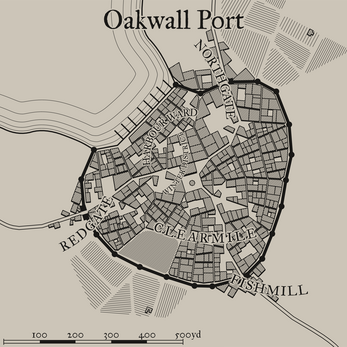
\includegraphics[height = 3 cm]{images/24FsvM.png}\\
     \captionof{figure}\small{Exemple de représentation d'une ville ancienne \\
    provenant de Medieval Fantasy City.}
\end{center}
}
{}
{
\begin{itemize}

\item \textbf{\tab Description : } Vérification que le fichier de sortie correspond à une nouvelle ville ayant pris en compte une génération d'une ancienne ville.\newline
\textbf{\tab Déroulement du test : } On lance le programme et on voit si on génère correctement une ville en ayant garder les anciens bâtiments déjà présents. \newline
\textbf{\tab Entrée : } Un programme de génération de ville aléatoire sur un plan déjà existant. \newline
\textbf{\tab Analyse du test : } Fonctionnement de la génération.

\item \textbf{\tab Description : }Vérification que le fichier de sortie respecte de nouveau les caractéristiques environnementales. \newline
\textbf{\tab Déroulement du test : } On essaie de mettre en place un bâtiment sur une zone qui n'est pas adaptée et on voit si ça fonctionne ou pas.\newline
\textbf{\tab Entrée : } Un programme de génération de ville.

\end{itemize}
}
\besoin{}
{\textcolor{cyan}{Fonctionnalités de l'interface}}
{
L'interface doit pouvoir donner à l'utilisateur l'éventualité de visualiser les éléments de la ville.
\\Dès le lancement il y aura un champs associé à chaque élément de la ville permettant de choisir les spécificités de la ville souhaitée,
en commençant par le nombre de routes principales,  le nombre de structures clés, le nombre de bâtiments et leurs types,
le nombre de montagnes, rivières, lacs et de collines, une fois ces éléments pris en compte, une ville se générera aléatoirement respectant les informations d'entrée.

\begin{itemize}
    \item Posséder un curseur temporel pour observer l'évolution de la ville au cours du temps, c'est à dire que la ville doit s'adapter en fonction de la période choisie par l'utilisateur.
    \item Avoir la possibilité de regénérer une nouvelle ville en écrasant l'ancienne
    \item Avoir la possibilité de choisir les paramètres des éléments, avant la génération de la ville.
    \item Un récapitulatif des données d'entrée.

\end{itemize}
}
{}
{
\begin{itemize}

  \item \textbf{Description : } Vérification que le fichier de sortie correspond à une interface manipulable par l'utilisateur.\newline
  \textbf{Déroulement du test : } On lance le programme et on voit si on génère correctement une interface. \newline
  \textbf{Entrée : } Un programme générant une interface pour l'utilisateur. \newline
  \textbf{ Analyse du test : } Fonctionnement de l'interface.
  
  \item \textbf{ Description : }Vérification que l'interface possède des boutons fonctionnels et impacte la génération de la ville. \newline
  \textbf{Déroulement du test : } On teste le fonctionnement des boutons utilisables sur l'interface. \newline
  \textbf{ Entrée : } Un programme générant une interface pour l'utilisateur.

  \item \textbf{ Description : }Vérification que l'interface prends bien en compte les données d'entrée \newline
  \textbf{Déroulement du test : } On génère des villes avec plusieurs données d'entrée. \newline
  \textbf{ Entrée : } Un jeu de données qu'on rentre dans les différents champs de l'interface. \newline
  \textbf{ Analyse du test : } On vérifie si l'affichage est correct, si les villes dont les données sont les mêmes ont des résultats similaires.
\end{itemize}
}